   
\documentclass[11pt]{article}
\renewcommand{\baselinestretch}{1.05}
\usepackage{amsmath,amsthm,verbatim,amssymb,amsfonts,amscd, graphicx}
\usepackage{mathtools}
\usepackage[table,xcdraw]{xcolor}
\DeclarePairedDelimiter{\ceil}{\lceil}{\rceil}
\usepackage{graphics}
\usepackage{enumitem}
\usepackage[table]{xcolor}
\usepackage{floatrow}
\usepackage{geometry}
\usepackage{tikz}
\usetikzlibrary{shapes.geometric,arrows,fit,matrix,positioning}
\tikzset
{
    treenode/.style = {rectangle, draw=black, align=center, minimum size=1cm},
    subtree/.style  = {isosceles triangle, draw=black, align=center, minimum height=0.5cm, minimum width=1cm, shape border rotate=90, anchor=north}
}
\topmargin0.0cm
\headheight0.0cm
\headsep0.0cm
\oddsidemargin0.0cm
\textheight23.0cm
\textwidth16.5cm
\footskip1.0cm
\theoremstyle{plain}
\newtheorem{theorem}{Theorem}
\newtheorem{corollary}{Corollary}
\usepackage{clrscode}
\newtheorem{lemma}{Lemma}
\newtheorem{proposition}{Proposition}
\newtheorem*{surfacecor}{Corollary 1}
\newtheorem{conjecture}{Conjecture} 
\newtheorem{question}{Question} 
\theoremstyle{definition}
\newtheorem{definition}{Definition}

\newlist{pcases}{enumerate}{1}
\setlist[pcases]{
  label=\underline{Case~\arabic*:}\protect\thiscase.~,
  ref=\arabic*,
  align=left,
  labelsep=0pt,
  leftmargin=0pt,
  labelwidth=0pt,
  parsep=0pt
}
\newcommand{\case}[1][]{%
  \if\relax\detokenize{#1}\relax
    \def\thiscase{}%
  \else
    \def\thiscase{~#1}%
  \fi
  \item
}
\usepackage{listings}
\usepackage{color}

\definecolor{dkgreen}{rgb}{0,0.6,0}
\definecolor{gray}{rgb}{0.5,0.5,0.5}
\definecolor{mauve}{rgb}{0.58,0,0.82}

\lstset{frame=tb,
  language=Java,
  aboveskip=3mm,
  belowskip=3mm,
  showstringspaces=false,
  columns=flexible,
  basicstyle={\small\ttfamily},
  numbers=none,
  numberstyle=\tiny\color{gray},
  keywordstyle=\color{blue},
  commentstyle=\color{dkgreen},
  stringstyle=\color{mauve},
  breaklines=true,
  breakatwhitespace=true
  tabsize=3
}
\newcommand{\blank}[1]{\hfil\penalty1000\hfilneg\rule[-3pt]{#1}{0.4pt}}
\begin{document}
 


\title{Algorithms and Data Structures on Arrays}
\author{By Joshua Kirstein (joshkirstein@ufl.edu)}
\maketitle

\section{Range Sum Query (RSQ)}
This set of notes will be framed around the Range Sum Query problem. Unlike in traditional problems where you are given one piece of input and are expected to produce one piece of output, \emph{query problems} are a class in which you are given some data as well as a set of questions (read: queries) on this data; for these problems, you have to design a solution which also factors in the amount of queries that will be given as it is typically very large. The \emph{Range Sum Query problem} is one such problem. For the Range Sum Query problem you are given an array of numbers $A[1 \dots n]$, and are expected to answer the following query:
$$\boxed{sum(i, j) = A[i] + A[i+1] + ... + A[j]}$$
Simply put, the answer to a range sum query is just the sum of every element between (and including) $A[i]$ and $A[j]$. If $A = [1, -2, 3, 5, 8, -5]$, then $sum(2, 4) = 6$ and $sum(2, 6) = 9$. The most naive algorithm takes $O(n)$ time per query, but can we do better?
\section{Take one: the method of prefix sums (steady accumulation)}
To tackle the RSQ problem, we will look at it from three different perspective which all rely on transforming the data into a new data structure. When analyzing solutions that rely on data structures, in addition to accounting for the run-time of a single query, we must also analyze the run-time associated with building that data structure (since it is often non-trivial). The plus-side to using data structures (as opposed to just an algorithm) is that building the data-structure is a one time cost that could potentially reduce the run-time of each query.\\\\
To leverage this type of power we will create a new array $B[1...n]$ that will serve as our data structure. The basic idea is that each element of this new array will store the \emph{prefix sum ending at i}, which is just the sum of every element before (and including) element $i$ --- that is $B[i] = A[1] + A[2] + \dots + A[i]$. But... how does this data structure help us solve the problem? Consider the following diagram:

\begin{figure}[h]
\centering
\caption{$B[7] - B[3] = A[4] + A[5] + A[6] + A[7]$}
\begin{tabular}{|
>{\columncolor[HTML]{34FF34}}c |
>{\columncolor[HTML]{34FF34}}c |
>{\columncolor[HTML]{34FF34}}c |
>{\columncolor[HTML]{34FF34}}c |
>{\columncolor[HTML]{34FF34}}c |
>{\columncolor[HTML]{34FF34}}c |
>{\columncolor[HTML]{34FF34}}c |c|c|}
\hline
A{[}1{]} & A{[}2{]} & A{[}3{]} & A{[}4{]} & A{[}5{]} & A{[}6{]} & A{[}7{]} & A{[}8{]} & A{[}9{]} \\ \hline
\end{tabular}
\begin{tabular}{|
>{\columncolor[HTML]{FE0000}}c |
>{\columncolor[HTML]{FE0000}}c |
>{\columncolor[HTML]{FE0000}}c |c|c|c|c|c|c|}
\hline
A{[}1{]} & A{[}2{]} & A{[}3{]} & A{[}4{]} & A{[}5{]} & A{[}6{]} & A{[}7{]} & A{[}8{]} & A{[}9{]} \\ \hline
\end{tabular}
\begin{tabular}{|c|c|c|
>{\columncolor[HTML]{38FFF8}}c |
>{\columncolor[HTML]{38FFF8}}c |
>{\columncolor[HTML]{38FFF8}}c |
>{\columncolor[HTML]{38FFF8}}c |c|c|}
\hline
A{[}1{]} & A{[}2{]} & A{[}3{]} & A{[}4{]} & A{[}5{]} & A{[}6{]} & A{[}7{]} & A{[}8{]} & A{[}9{]} \\ \hline
\end{tabular}
\end{figure}




\newpage \noindent If it isn't obvious now, observe that $$B[j] - B[i-1] = (A[1] + A[2] + \dots + A[j]) - (A[1] + A[2] + \dots + A[i-1]) = A[i] + A[i+1] + \dots + A[j] = sum(i, j),$$ or put in a more revealing way $$\boxed{sum(i, j) = B[j] - B[i-1]}$$ What this means is that once we have computed $B[1...n]$, answering queries is as simple as two lookups in this array. Therefore we can compute a RSQ in $O(1)$ time assuming that we know what $B[1...n]$ looks like!!!! But how do we know what $B[1...n]$ looks like? The most obvious way to compute $B[1...n]$ is with an $O(n^2)$ algorithm which, for large $n$, is pretty terrible. I'll leave it as an exercise to figure out how to compute it in $O(n)$ (\emph{hint:} notice that $B[i] = A[i] + B[i-1]$).\\\\ ...and with that we've created our first data structure to solve the RSQ problem with the following time complexities:
\begin{center}
\fbox{\begin{minipage}{11.339em}
Pre-processing time: $O(n)$\\
\hspace{-15mm}Query time: $O(1)$
\end{minipage}
}
\end{center}
**Again** note that, since the pre-processing step happens only once, this solution is \emph{much} faster than the most naive one.
\section{Take two: square root decomposition}
It turns out that the method we just developed is the absolute best we can do (can you form an argument as to why it is?). What if, in addition to supporting the query $sum(i, j)$, we wanted to allow the following operation as well: $$\boxed{set(i, v) :=\text{ set the value of }A[i]  \text{ to } v}$$
Here we're allowed any number of $set()$ operations intermixed with $sum()$ queries, and we want to support them in the fastest way possible. It turns out that adding this operation increases the number of solutions to this problem but also kills the method of prefix sums. \\\\ Preempting the conclusion to this section, we will be designing a data structure which supports the operations with the following run-times:
\begin{center}
\fbox{\begin{minipage}{11.5em}
Pre-processing time: $O(n)$\\
\hspace{-15mm}$sum(i,j)$ time: $O(\sqrt{n})$\\
\hspace{-15mm}$set(i,v)$ time: $O(\sqrt{n})$
\end{minipage}
}
\end{center}
It's pretty weird to see the square root function appear in a run-time analysis, but there is a special property that makes it appealing: $\sqrt{n} \times \sqrt{n} = n$.
\subsection{The data structure}
The basic idea is to cut the original array into consecutive pieces of size $\sqrt{n}$ (or roughly of size $\sqrt{n}$ if $n$ is not a perfect square) and store, for each piece, the sum of the elements inside of it. Assuming we know how to compute $sum(i, j)$ from this information, updating the data structure (i.e., the set operation) is as easy as recomputing the sum of the piece that the element being updated is a part of.\\\\
%INSERT PIC
Unfortunately it's not possible to explain this data structure without some notation (also, so we don't have to handle any special cases, we assume that $n$ is a perfect square). With that being said, first cut the original array given into chunks of size $\sqrt{n}$. Next, assign each chunk an index between $1$ and $\sqrt{n}$ where the first chunk gets assigned index 1, the second chunk gets assigned index 2, and so on, with the final chunk being assigned index $\sqrt{n}$. Then, our data structure is the array $B[1...\sqrt{n}]$ defined as follows:
$$\boxed{B[i] := \text{sum of the elements in chunk \emph{i}}}$$ The naive method of going through each element in each chunk and summing them in order to compute $B[1...\sqrt{n}]$ is optimal. Since there are $\sqrt{n}$ chunks each with $\sqrt{n}$ elements, in total building the data structure takes $O(\sqrt{n} \times \sqrt{n}) = O(n)$ time.\\\\
At this point it doesn't seem obvious where we're going with this. How does this data structure allow us to compute a RSQ fast?
\subsection{A quick example}
Consider the following array given as input (remember, we're doing every 1-indexed):

\begin{table}[h]
\centering
\begin{tabular}{|l|l|l|l|l|l|l|l|l|}
\hline
-3 & 7 & 5 & 8 & 2 & -1 & 6 & 3 & 2 \\ \hline
\end{tabular}
\end{table}
\noindent Since $\sqrt{9} = 3$, we decompose this array into contiguous pieces of size $3$:
\begin{table}[h]
\centering
\begin{tabular}{|
>{\columncolor[HTML]{FF0000}}c |
>{\columncolor[HTML]{FF0000}}c |
>{\columncolor[HTML]{FF0000}}c |
>{\columncolor[HTML]{00BCFF}}c |
>{\columncolor[HTML]{00BCFF}}c |
>{\columncolor[HTML]{00BCFF}}c |
>{\columncolor[HTML]{00FF07}}c |
>{\columncolor[HTML]{00FF07}}c |
>{\columncolor[HTML]{00FF07}}c |}
\multicolumn{3}{c}{Chunk: 1} & \multicolumn{3}{c}{Chunk: 2} & \multicolumn{3}{c}{Chunk: 3} \\
\multispan3\mathstrut\downbracefill & \multispan3\mathstrut\downbracefill  & \multispan3\mathstrut\downbracefill \vspace{+1.5mm}

\\
\hline
-3 & 7 & 5 & 8 & 2 & -1 & 6 & 3 & 2 \\ \hline
\multispan3\mathstrut\upbracefill & \multispan3\mathstrut\upbracefill  & \multispan3\mathstrut\upbracefill  \\
\multicolumn{3}{c}{B[1] = 9} & \multicolumn{3}{c}{B[2] = 9} & \multicolumn{3}{c}{B[3] = 11} \\
\end{tabular}
\end{table}
\subsection{sum in $O(\sqrt{n})$}
So now let's assume that we have already constructed the array $B[1...\sqrt{n}]$ and we want to compute $sum(i, j)$. How can we do this? Let's take a look at an array of length 16 and try and compute $sum(3, 15)$.
\begin{table}[h]
\centering
\begin{tabular}{|
>{\columncolor[HTML]{FF0000}}c |
>{\columncolor[HTML]{FF0000}}c |
>{\columncolor[HTML]{00BCFF}}c |
>{\columncolor[HTML]{00BCFF}}c |
>{\columncolor[HTML]{00FF07}}c |
>{\columncolor[HTML]{00FF07}}c |
>{\columncolor[HTML]{00FF07}}c |
>{\columncolor[HTML]{00FF07}}c |
>{\columncolor[HTML]{00FF07}}c |
>{\columncolor[HTML]{00FF07}}c |
>{\columncolor[HTML]{00FF07}}c |
>{\columncolor[HTML]{00FF07}}c |
>{\columncolor[HTML]{00BCFF}}c |
>{\columncolor[HTML]{00BCFF}}c |
>{\columncolor[HTML]{00BCFF}}c |
>{\columncolor[HTML]{FF0000}}c |}
\hline
-3 & 5 & 6 & 2 & 3 & -1 & 7 & 9 & 12 & 6 & 2 & 3 & 5 & 4 & 5 & -10 \\ \hline
\multispan4\mathstrut\upbracefill & \multispan4\mathstrut\upbracefill  & \multispan4\mathstrut\upbracefill  & \multispan4\mathstrut\upbracefill  \\
\multicolumn{4}{c}{B[1] = 10} & \multicolumn{4}{c}{B[2] = 18} & \multicolumn{4}{c}{B[3] = 23} & \multicolumn{4}{c}{B[4] = 4} \\
\end{tabular}
\end{table}
\\
To compute $sum(3, 15)$ we're going to go through each of the $\sqrt{n}$ chunks and figure out how much each one contributes to it. There are two important things to notice when going down this line of thought. First, $B[1]$ and $B[4]$ are not very useful because they contain numbers that are not part of the sum ($A[1]$ and $A[2]$ are contained in $B[1]$; $A[16]$ is contained in $B[4]$). Second,  $B[2]$ and $B[3]$ contain elements that are \emph{completely} inside the sum. Why are these two facts useful? The second fact tells us that we don't really need to worry about what the individual elements inside chunk 2 and 3 are --- since they are fully contained within $sum(3, 15)$ all we care about are the sums $B[2]$ and $B[3]$. The first fact tells us that we \emph{can't} just say $sum(3, 15) = B[1] + B[2] + B[3] + B[4]$ and call it a day, since both $B[1]$ and $B[4]$ contain the sum of elements we don't want. This way we view the sum as
$$\boxed{sum(3, 15) = (A[3] + A[4]) + (B[2] + B[3] ) + (A[13] + A[14] + A[15])}$$
which motivates the following algorithm
\begin{lstlisting}
function sum(i, j):
sum = 0
foreach chunk c 
	if chunk c is completely contained within (i, j)
		// since this chunk is completely contained within
		// the sum, we just add the precomputed sum B[c]
		sum += B[c]
	else if chunk c is partially contained within (i, j)
		// go through each element in this chunk
		// and add the ones we care about to the sum
		foreach index e in chunk c
			if index e is within (i, j)
				sum += A[e]
			endif
		endfor
	else 
		// chunk doesn't contain any element in sum(i, j)
		// so we just ignore it
	endif
endfor
return sum
\end{lstlisting}

\noindent The proof that the run-time is $O(\sqrt{n})$ is the key to why this works, but at first it may seem tricky to reason out. The basic idea is to figure how many times each branch of the if statement is executed, and multiply that with their respective costs to get the total run-time of the algorithm. With that in mind, look at the following pseudocode annotated with the run-time of each branch of the if statement.

\begin{lstlisting}[mathescape=true]
foreach chunk c 
	if chunk c is completely contained within (i, j)
		$+\ O(1)$
	else if chunk c is partially contained within (i, j)
		$+\ O(\sqrt{n})$
	else 
		$+\ O(1)$
	endif
endfor
\end{lstlisting}
All we have to do now is figure out how many times each branch is executed... How many chunks satisfy the condition 'chunk c is completely contained within (i, j)'? At most $O(\sqrt{n})$. How many chunks satisfy the condition 'chunk c is partially contained within (i, j)'? If you think about it, only $2$ chunks can satisfy this condition! Finally, how many chunks can satisfy neither of these conditions (i.e., the third branch of the if statement)? At most $O(\sqrt{n})$. Thus,
$$\boxed{\text{Run-time} = O(\sqrt{n}) * O(1) + 2*O(\sqrt{n}) + O(\sqrt{n})*O(1) = O(\sqrt{n})}$$
\subsection{set in $O(\sqrt{n})$}
Supporting the $set(i, v)$ operation is as simple as recomputing $B[j]$ (where $j$ is the index of the chunk $A[i]$ is a part of) after we set $A[i] = v$. This can easily be done in $O(\sqrt{n})$ (just sum every element in the chunk... there are $\sqrt{n}$ of them).
\section{Take three: fenwick trees (logarithmic accumulation)}
TODO: Hmm, just go to segment trees.
\section{Final take: segment trees}
The benefit of square root decomposition is that it's conceptually fairly simple; honestly though, it's a burden to code if you've never done it before and it turns out that it isn't \emph{very} fast, which is what we really want. Fenwick trees are slightly more challenging conceptually, but turn out to be asymptotically optimal (actually the build time of a Fenwick tree is slightly worse) and one of the easiest data structures to implement. So why don't we always use a Fenwick tree? Well, Fenwick trees only work on the RSQ problem... meaning they can't really be applied to any other type of query problem. What if, instead of asking for the sum between elements $A[i]$ and $A[j]$, we want to find the \emph{largest} element between them? Good luck trying to modify a Fenwick tree to do that!\\\\
In this section we design a data structure which achieves the same run-time bounds as a Fenwick tree, but with the added benefit that it can be applied to many different type of query problems on arrays (bad news is, it's not as easy to code). 
\subsection{The data structure: conceptual}
Our first step toward achieving a logarithmic run-time bound is to try and look at the array provided as a binary tree. With that being said, we're going to construct a binary tree where each node represents some consecutive sequence in the array. This could be the sequence $[0, n-1]$ (the whole array), $[2, 3]$ (the 3rd and 4th elements), etc. In every binary tree, a node has to have around two children. What do the children of our nodes look like? Well, consider the following diagram:
\begin{figure}[h]
    \caption{How to split a node into children.}
\centering

{
    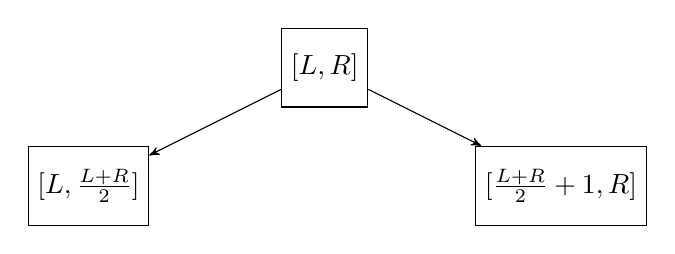
\begin{tikzpicture}[->,>=stealth', level/.style={sibling distance = 6cm/#1, level distance = 1.5cm}, scale=1,transform shape]
    \node [treenode] {$[L, R]$}
    child
    {
        node [treenode] {$[L, \frac{L+R}{2}]$} 
    }
    child
    {
        node [treenode] {$[\frac{L+R}{2}+1, R]$} 
    }
;
\end{tikzpicture}
}
\end{figure}
\\ \\ \\ \\ \\ \\ \\
Here we're looking at a node that corresponds to the interval $[L, R]$ and split it up into two (roughly equal) sequences which become its two children. The root of our segment tree corresponds to the whole array (i.e., segment $[0, n-1]$). From these two pieces of information we can construct a segment tree as follows:\\
\\starting from the root ($[0, n-1]$) we split its segment into two children c1 ($[0, \frac{n-1}{2}]$) and c2 $([\frac{n-1}{2}+1, n])$.
\\ \indent for each one of those children, in turn, we split it with the same process
\\ \indent \indent for each one of the children's children, we split it with the same process
\\ \indent \indent \indent ... until we can't split the segments anymore (i.e., the segments are length 1)
\\\\
Here is the segment tree for the ($n=10$) array $[5, -3, 8, 2, 6, 3, -4, -1, 1, 2]$ (note that we store the sum of each node's segment inside of the node):
\begin{figure}[h]
\caption{The segment tree corresponding to the array $[5, -3, 8, 2, 6, 3, -4, -1, 1, 2]$}
\centering
{
    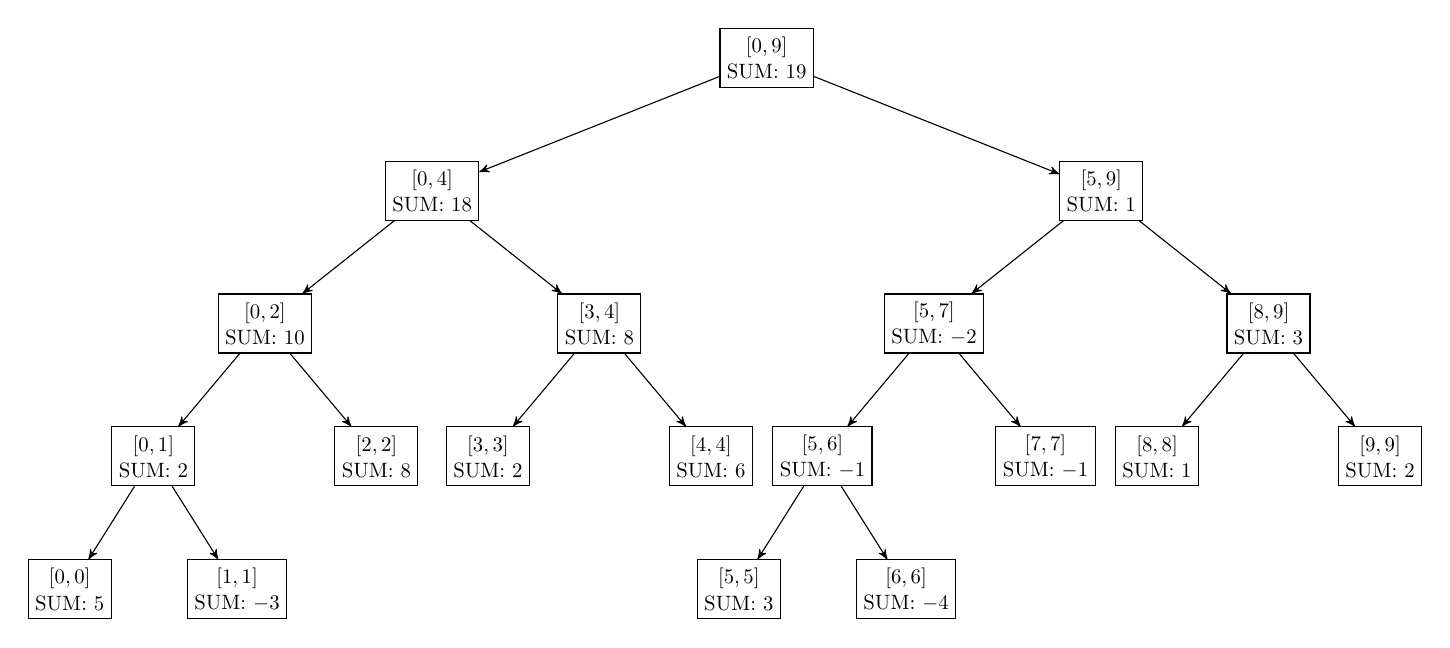
\begin{tikzpicture}[->,>=stealth', level/.style={sibling distance = 11.33cm/#1, level distance = 2.25cm}, scale=0.75,transform shape]
    \node [treenode] {$[0, 9]$ \\ SUM: $19$}
    child
    {
        node [treenode] {$[0, 4]$ \\ SUM: $18$} 
        child
        {
             node [treenode] {$[0, 2]$ \\ SUM: $10$} 
             child
             {
                  node [treenode] {$[0, 1]$ \\ SUM: $2$} 
                  child
                  {
                       node [treenode] {$[0, 0]$ \\ SUM: $5$} 
                  }
                  child
                  {
                       node [treenode] {$[1, 1]$ \\ SUM: $-3$} 
                  }
             }
             child
             {
                  node [treenode] {$[2, 2]$ \\ SUM: $8$} 
             }
        }
        child
        {
             node [treenode] {$[3, 4]$ \\ SUM: $8$} 
             child
             {
                  node [treenode] {$[3, 3]$ \\ SUM: $2$} 
             }
             child
             {
                  node [treenode] {$[4, 4]$ \\ SUM: $6$} 
             }
        }
    }
    child
    {
        node [treenode] {$[5, 9]$ \\ SUM: $1$} 
        child
        {
             node [treenode] {$[5, 7]$ \\ SUM: $-2$} 
             child
             {
                  node [treenode] {$[5, 6]$ \\ SUM: $-1$} 
                  child
                  {
                       node [treenode] {$[5, 5]$ \\ SUM: $3$} 
                  }
                  child
                  {
                       node [treenode] {$[6, 6]$ \\ SUM: $-4$} 
                  }
             }
             child
             {
                  node [treenode] {$[7, 7]$ \\ SUM: $-1$} 
             }
        }
        child
        {
             node [treenode] {$[8, 9]$ \\ SUM: $3$} 
             child
             {
                  node [treenode] {$[8, 8]$ \\ SUM: $1$} 
             }
             child
             {
                  node [treenode] {$[9, 9]$ \\ SUM: $2$} 
             }
        }
    }
;
\end{tikzpicture}
}
\end{figure}
\\\\
Which looks totally cool and all, but it raises soooooo many questions:
\\\\
(1) How can we store this data structure so that it's easy to use? \\\\
(2) How do we physically build this data structure?\\\\
(3) Why is this data structure even useful?\\\\
\\\\
\noindent These questions will all soon be answered. But before, an important fact about segment trees must be mentioned:
$$\boxed{\text{The height (number of layers) in a segment tree is } O(\log_2{n})}$$
\subsection{The data structure: practical aspects}
In this subsection we will first describe how to store a segment tree in memory and then how to build it. It turns out that there are quite a few ways to represent binary trees in memory. The method adopted by the competitive programming community is very similar to how \emph{heapsort} works.\\\\
Take a look at figure 3 above. Notice how the last level isn't completely filled because the size of the array isn't a perfect power of 2. Just to illustrate how we're going to store this tree in memory, we're going to \emph{fill} the last layer with \emph{dummy nodes} so that the segment tree becomes a \emph{perfect binary tree}; it's important to keep in mind that we don't really care about these nodes, but they're important to demonstrate how we're going to store this tree. Next, we systematically assign an index to each node. Start by assigning the root node an index of 0, then move down to the next level and assign nodes consecutive values from left to right. Repeat for the next level (and levels after) until every node is assigned an index. This can be seen as the root node getting index `0', its left-most child getting index `1' and its right-most child gets index `2'. Continuing this we get an arrangement that looks like (the dummy nodes aren't pictured here because it's SO difficult to make the graph fit):
\begin{figure}[h]
\caption{The indices of each node in the segment tree.}
\centering
{
    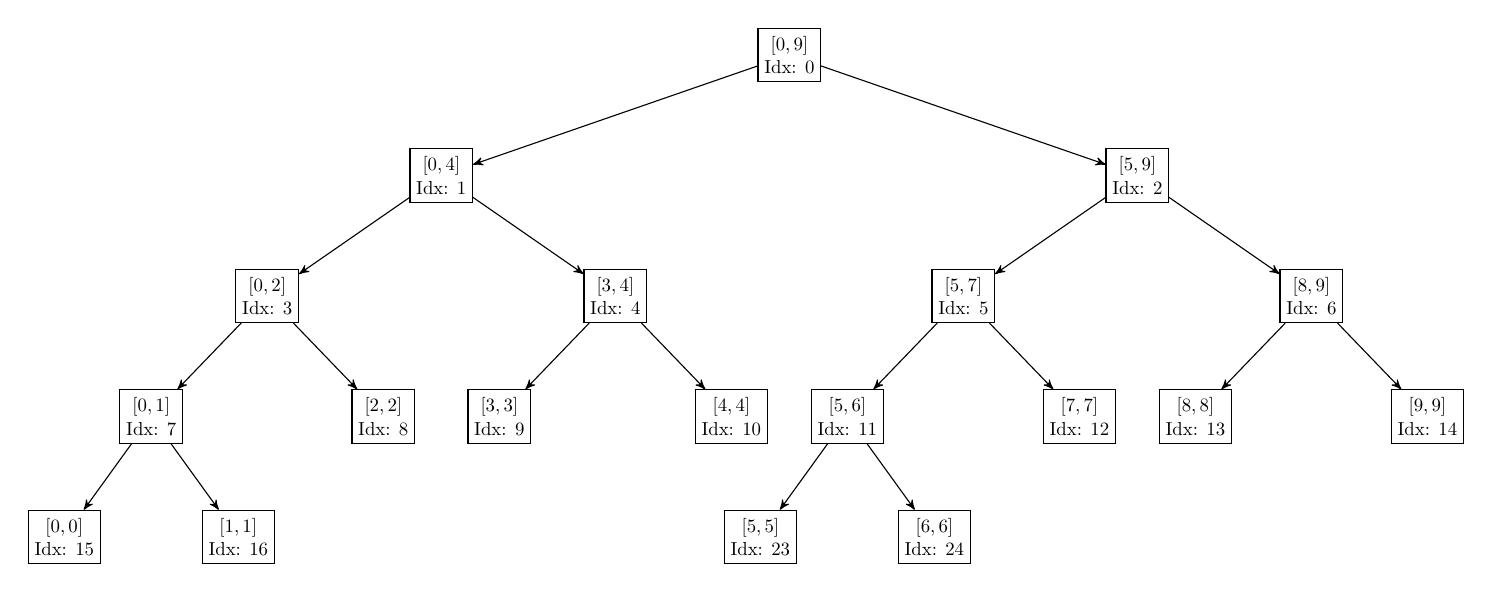
\begin{tikzpicture}[->,>=stealth', level/.style={sibling distance = 13cm/#1, level distance = 2.25cm}, scale=0.68,transform shape]
    \node [treenode] {$[0, 9]$ \\ Idx: 0}
    child
    {
        node [treenode] {$[0, 4]$ \\ Idx: 1} 
        child
        {
             node [treenode] {$[0, 2]$ \\ Idx: 3} 
             child
             {
                  node [treenode] {$[0, 1]$ \\ Idx: 7} 
                  child
                  {
                       node [treenode] {$[0, 0]$ \\ Idx: 15} 
                  }
                  child
                  {
                       node [treenode] {$[1, 1]$ \\ Idx: 16} 
                  }
             }
             child
             {
                  node [treenode] {$[2, 2]$ \\ Idx: 8} 
             }
        }
        child
        {
             node [treenode] {$[3, 4]$ \\ Idx: 4} 
             child
             {
                  node [treenode] {$[3, 3]$ \\ Idx: 9} 
             }
             child
             {
                  node [treenode] {$[4, 4]$ \\ Idx: 10} 
             }
        }
    }
    child
    {
        node [treenode] {$[5, 9]$ \\ Idx: 2} 
        child
        {
             node [treenode] {$[5, 7]$ \\ Idx: 5} 
             child
             {
                  node [treenode] {$[5, 6]$ \\ Idx: 11} 
                  child
                  {
                       node [treenode] {$[5, 5]$ \\ Idx: 23} 
                  }
                  child
                  {
                       node [treenode] {$[6, 6]$ \\ Idx: 24} 
                  }
             }
             child
             {
                  node [treenode] {$[7, 7]$ \\ Idx: 12} 
             }
        }
        child
        {
             node [treenode] {$[8, 9]$ \\ Idx: 6} 
             child
             {
                  node [treenode] {$[8, 8]$ \\ Idx: 13} 
             }
             child
             {
                  node [treenode] {$[9, 9]$ \\ Idx: 14} 
             }
        }
    }
;
\end{tikzpicture}
}
\end{figure}
\\ \noindent At this point (probably if you've never seen this before) you may be wondering why we're doing the assignment of indices this way. First off, it let's us `flatten' the tree and store it in a one-dimensional array. $tree[0]$ will store the data for the root, $tree[1]$ will store the data for the root's left-most child, and so on. The `data' that we're worried about is the sum of the segment corresponding to the node (the `SUM' values in figure 1). Second, it has the nice property that, if a node's index is $x$, then its left child's index is $2x+1$ and its right child's index is $2x+2$; this property will turn out to be very useful later on. Oh man!!!!!! NOW WE'RE READY TO CONSTRUCT A SEGMENT TREE:
\begin{lstlisting}
class SegmentTree {
	//backing array
	int[] array;
	//length of the array
	int n;
	//this will store the sum for each node
	int[] tree;
	//stores the left endpoint of each node
	int[] left;
	//stores the right endpoint of each node
	int[] right;
	
	//construct a segment tree for the array
	SegmentTree(int[] array) {
		this.array = array;
		n = array.length;
		tree = new int[4*n];
		left = new int[4*n];
		right = new int[4*n];
		build(0, 0, n-1);
	}

	//recursively build the tree
	//node_idx is the current nodes idx
	//node_left and node_right are the left
	//and right endpoints of the current node's segment
	void build(int node_idx, int node_left, int node_right) {
		left[node_idx] = node_left;
		right[node_idx] = node_right;
		if (node_left == node_right) {
			//base case, the segment can't be
			//split anymore!!!!!!!!!!!
			tree[node_idx] = array[node_left];
		} else {
			//recursively build the children
			build(2*node_idx+1, node_left, (node_left+node_right)/2);
			build(2*node_idx+2, (node_left+node_right)/2+1, node_right);
			//we still need to compute tree[node_idx].
			//observe that the tree[idx] = tree[leftidx]+tree[rightidx]
			//(i.e., we're just taking the sum of the left and right children)
			tree[node_idx] = tree[2*node_idx+1] + tree[2*node_idx+2];
		}
	}
}
\end{lstlisting}
\newpage \noindent
The code is hopefully commented enough to be self-describing. There is actually one trick that goes into constructing the segment tree: `tree = new int[4*n]'. What's with the use of `4*n'? This basically says that, if we build a segment tree on an $n$-dimensional array, that we'll never have a node whose index is larger than $4*n$. Remember how we had to introduce dummy nodes to index the tree? Even though they don't physically exist, their spot in memory does and we're not allowed to remove them; making the `tree' array size $4*n$ guarantees that all of our node indices will fit in this array by accounting for the dummy nodes. \\\\ 
Since there are only $4*n = O(n)$ nodes, it's not too hard to see that the run-time of this build procedure is $O(n)$.
\subsection{sum in $O(\log_2{n})$}
Just as with the sum query for square root decomposition, our goal for computing $sum(i, j)$ is to represent the desired value as the sum of values in our data structure. Before we dive into the general method for computing a sum, let's take a look at an example. Using the segment tree we computed above, let's try and figure out the nodes which constitute the value of $sum(1, 8)$.
\begin{figure}[h]
\caption{Color coded segment tree of $[5, -3, 8, 2, 6, 3, -4, -1, 1, 2]$ corresponding to $sum(1, 8)$!!!!}
\centering
{
    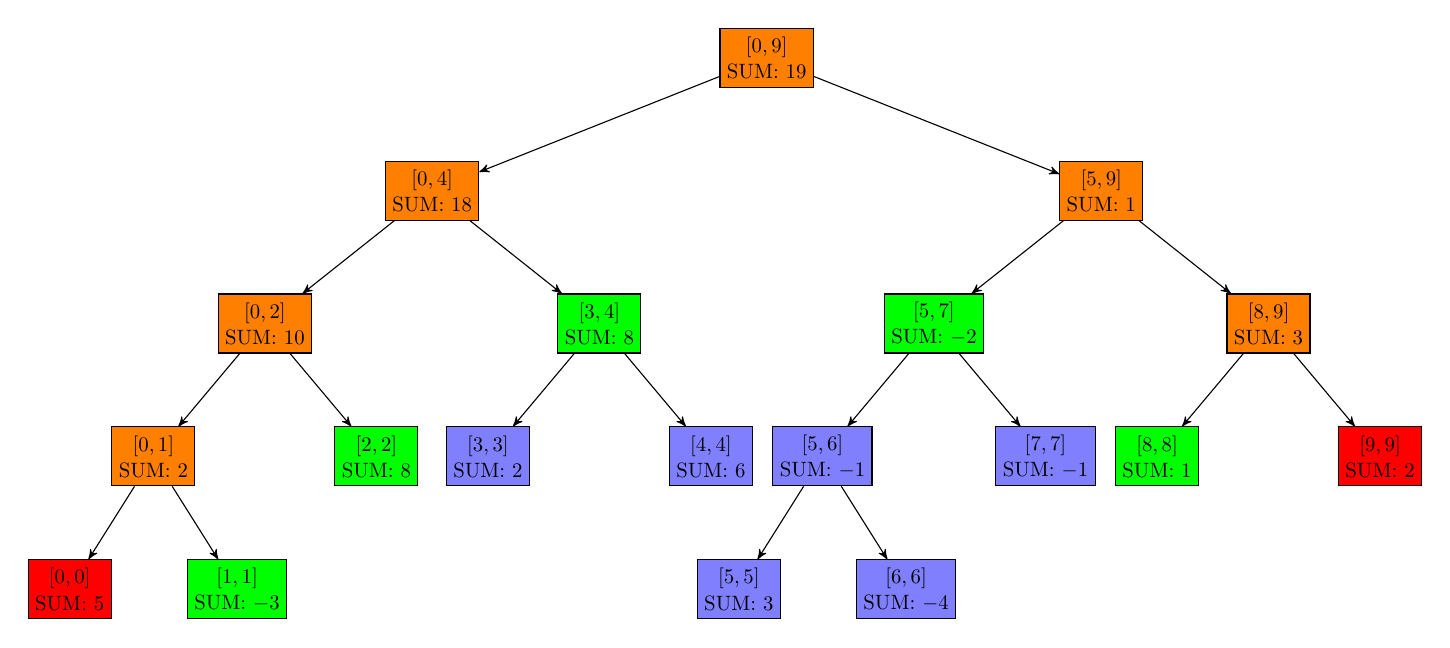
\begin{tikzpicture}[->,>=stealth', level/.style={sibling distance = 11.33cm/#1, level distance = 2.25cm}, scale=0.75,transform shape]
    \node [treenode,fill=orange] {$[0, 9]$ \\ SUM: $19$}
    child
    {
        node [treenode,fill=orange] {$[0, 4]$ \\ SUM: $18$} 
        child
        {
             node [treenode,fill=orange] {$[0, 2]$ \\ SUM: $10$} 
             child
             {
                  node [treenode,fill=orange] {$[0, 1]$ \\ SUM: $2$} 
                  child
                  {
                       node [treenode,fill=red] {$[0, 0]$ \\ SUM: $5$} 
                  }
                  child
                  {
                       node [treenode,fill=green] {$[1, 1]$ \\ SUM: $-3$} 
                  }
             }
             child
             {
                  node [treenode,fill=green] {$[2, 2]$ \\ SUM: $8$} 
             }
        }
        child
        {
             node [treenode,fill=green] {$[3, 4]$ \\ SUM: $8$} 
             child
             {
                  node [treenode,fill=blue!50] {$[3, 3]$ \\ SUM: $2$} 
             }
             child
             {
                  node [treenode,fill=blue!50] {$[4, 4]$ \\ SUM: $6$} 
             }
        }
    }
    child
    {
        node [treenode,fill=orange] {$[5, 9]$ \\ SUM: $1$} 
        child
        {
             node [treenode,fill=green] {$[5, 7]$ \\ SUM: $-2$} 
             child
             {
                  node [treenode,fill=blue!50] {$[5, 6]$ \\ SUM: $-1$} 
                  child
                  {
                       node [treenode,fill=blue!50] {$[5, 5]$ \\ SUM: $3$} 
                  }
                  child
                  {
                       node [treenode,fill=blue!50] {$[6, 6]$ \\ SUM: $-4$} 
                  }
             }
             child
             {
                  node [treenode,fill=blue!50] {$[7, 7]$ \\ SUM: $-1$} 
             }
        }
        child
        {
             node [treenode,fill=orange] {$[8, 9]$ \\ SUM: $3$} 
             child
             {
                  node [treenode,fill=green] {$[8, 8]$ \\ SUM: $1$} 
             }
             child
             {
                  node [treenode,fill=red] {$[9, 9]$ \\ SUM: $2$} 
             }
        }
    }
;
\end{tikzpicture}
}
\end{figure}
\\ \noindent Starting from the root, we traverse each node checking to see if it's relevant to the query $sum(1, 8)$. Red nodes contribute nothing, orange nodes are partially contained within $[1, 8]$, green nodes are completely contained within $[1, 8]$, and blue nodes are those which are completely contained within $[1, 8]$ but are already accounted for in a segment higher up in the tree. If we sum the values of the green nodes we get $sum(1, 8) = -3 + 8 + 8 - 2 + 1 = 12$, which is the correct value. There are a couple things to note: \\\\
(1) once we hit a red node, we don't care about looking at any of the nodes descending from it because a red node, by definition, contributes nothing and therefore its children don't
\\\\
(2) once we hit a green node, we don't care about looking at any of the nodes descending from it (why?) (because every descendant of a green node is a blue node, and by definition blue nodes have already been accounted for)
\\\\
(3) orange values are a bit of a mystery, but if you think really really hard it turns out that there can be at most two 'paths' of orange nodes. The first orange path leads to the left-most node green node and the other orange path leads to the right-most green node. (***THIS IS REALLY REALLY IMPORTANT***)
\\\\
(4) the parent of a red or green node is an orange node.
\\\\
These facts will become important soon. Facts (1) - (2) are used to speed up the algorithm we described above and facts (3) - (4) prove why our algorithm is fast. Just be on the lookout for that. :)
\\\\
Just as we did with the specific example of computing $sum(1, 8)$, our algorithm is essentially just going to traverse the whole tree and determine which nodes are `green', `red', `orange', or `blue. If a node is `green', we want to add it to our running sum; all other nodes we just ignore. The following Java code does exactly that:
\begin{lstlisting}
//this function serves as the 'driver' (or API)
//to our 'real_query' function
//query_left and query_right are just the endpoints
int query(int query_left, int query_right) {
	//initialize the real query starting at the root
	return real_query(0, query_left, query_right);
}

int real_query(int node_idx, int query_left, int query_right) {
	//determine the color of 'node_idx':
	//query_left <= left[node_idx] <= right[node_idx] <= query_right
	if (left[node_idx] >= query_left && right[node_idx] <= query_right) {
		//this means 'node_idx' is COMPLETELY contained
		//within the bounds of the query....(GREEN NODE)
		return tree[node_idx]; // using fact (2)
	}
	else if (left[node_idx] > query_right || right[node_idx] < query_left) {
		//this means `node_idx' does not contain anything
		//within the bounds of the query....(RED NODE)
		return 0; // using fact (1)
	} else {
		//otherwise, this node is partially contained within
		//the query bounds....(ORANGE NODE)

		//in this case, we can't really figure out what to return,
		//so we just recursively look at our children and have them figure it out
		return real_query(2*node_idx+1, query_left, query_right) +
				real_query(2*node_idx+2, query_left, query_right);
	}
}
\end{lstlisting}

\noindent I'll skip the technical details of determining the color of a node and just go straight to how we handle each color. When we hit a `red node,' fact (1) tells us that it and all of its descendants are irrelevant to our query; for this case, we can immediately stop our search and return `0' indicating that no contribution to the total sum is being made. When we hit a `green node,' fact (2) tells us that we don't need to consider any of the nodes descending from it, since they will be blue nodes and they're already accounted for by a green node, and that the sum of the green node needs to be added to the total sum, so we return it. Based on this previous statement, it turns out that this recursive function will \emph{never} be called on a blue node. Finally, when we hit an `orange node' we simply defer the decision of figuring out which nodes we want to add to the total sum to its children.
\\\\
At this point it may or may not be obvious that the run-time of this procedure, as it stands right now, is $O(\log_2{n})$. Why is it? In the worst case, our function will run a total of $X$ times (currently we don't know $X$, but we will in a second). Since each function call takes $O(1)$ to execute, the total run-time of the algorithm in the worst case is $X*O(1) = O(X)$. Okay, so I guess we're done.... jk, we don't really know what $X$ is. Can we express $X$ in terms of something we may know? If you think about it, $X = \text{\#red nodes} + \text{\#green nodes} + \text{\#orange nodes}$. Now recall this fact:

$$\boxed{\text{The height (number of layers) in a segment tree is } O(\log_2{n})}$$

\noindent In combination with fact (3), we learn that $\text{\#orange nodes} \leq 2*O(\log_2{n})$ (the boxed statement tells us that a path can't be longer than $O(\log_2{n})$ and fact (3) tells us that we have two paths of orange nodes). Finally, fact (4) tells us that $(\text{\#red nodes} + \text{\#green nodes}) \leq 2*\text{\#orange nodes}$ (I'll let you try and fully reason out why this is true using fact (4)).
\\\\
Combining this all together we get $X = \text{\#red nodes} + \text{\#green nodes} + \text{\#orange nodes} \leq 2*\text{\#orange nodes}  + \text{\#orange nodes} \leq 3*(2*O(\log_2{n}))$. Thus, $X = O(\log_2{n})$, giving us the correct run-time bound for our $sum()$ algorithm.

\subsection{set in $O(\log_2{n})$}
If you made it this far unfazed, the $set()$ operation should be no problem to figure out. Otherwise, here's a hint: solve it recursively just like we did for $sum()$ and figure out which nodes get affected by the set operation --- if you draw it out you'll notice that there's only one path of nodes that gets affected. The full segment tree code provided in the code appendix contains the $set()$ operation.
\section{Comments}
In this set of notes we covered four fundamental techniques to solve query problems on arrays (framed through the RSQ problem). It turns out that there are many other methods to solve these types of people. One class of them, known as \emph{offline algorithms}, take in all of the queries at once (instead of considering an individual query) and try to figure out the answer to all of them in one go. The quintessential example of an offline algorithm is \emph{Tarjan's offline lower common ancestor algorithm}. Another approach (which turns out to be very similar to Fenwick trees) is the idea of \emph{sparse table dynamic programming}.\\\\
More often than not, problems are asked where the data structures presented here are meant to \emph{augment} the solution in order to make it run faster.\\\\
Surprisingly, it's possible to support the so called \emph{range update} operation ($set(i, j, v)$ --- set all of the values between $A[i]$ and $A[j]$ to $v$) in $O(\log_2{n})$ via a method known as \emph{lazy propagation}. In an even more bizarre twist, it turns out that we can use two Fenwick trees to support the range update operation in $O(\log_2{n})$. \\\\
Although all of the data structures mentioned in this set of notes were framed around the RSQ problem, it is possible to modify some of them to handle different types of queries on arrays. The code for square root decomposition in the appendix actually solves the \emph{range minimum query} problem.
\section{Problems}
$$\boxed{\text{http://www.spoj.com/problems/CSUMQ/}}$$
$$\boxed{\text{http://codeforces.com/contest/380/problem/C}}$$
$$\boxed{\text{http://www.spoj.com/problems/RPLN/}}$$
$$\boxed{\text{https://uva.onlinejudge.org/external/112/11235.pdf}}$$
\section*{Code Appendix}
\subsection*{Square root decomposition}
This code is 0-indexed. Instead of solving the RSQ problem, this solves the RMQ problem (Range Minimum Query). Try writing the $set(i, v)$ operation!
\begin {lstlisting}
class RMQ {
	int[] array; // the array 'A'
	int[] sqrt; // the array 'B'

	RMQ(int[] array) {
		// on construction, pre-compute B
		this.array = array;
		int sq = (int) Math.ceil(Math.sqrt(array.length));
		this.sqrt = new int[sq+1];
		int j = 0;
		// j is the chunk index, i is the the first element
		// A[i] that is part of chunk j
		for (int i = 0; i < array.length; i += sq, j++) {
			int end = Math.min(array.length-1, i+sq-1);
			int min = Integer.MAX_VALUE;
			for (int k = i; k <= end; k++) {
				min = Math.min(min, array[k]);
			}
			sqrt[j] = min;
		}
	}

	// find the min between A[l] ... A[r]
	int query(int l, int r) {
		int sq = (int)  Math.ceil(Math.sqrt(array.length));
		int j = 0;
		int min = Integer.MAX_VALUE;
		// go through each chunk (chunk index is j)
		for (int i = 0; i < array.length; i += sq, j++) {
			// chunk j is responsible for A[lo] ... A[hi]
			int lo = i;
			int hi = i+sq-1;
			if (lo >= l && hi <= r) {
				// chunk completely contained
				min = Math.min(min, sqrt[j]);
			} else {
				// chunk partially contained,
				// only go through elements that we care about
				int x=-1, y=-1;
				if (l >= lo && r > hi) {
					x = l;
					y = r;
				} else if (r <= hi && l < lo) {
					x = lo;
					y = r;
				} else if (l >= lo && r <= hi) {
					x = l;
					y = r;
				}
				if (x != -1 && y != -1) {
					// if x != -1 and y != -1, this chunk contains 
					// elements we care about
					for (int k = x; k <= y; k++) {
						min = Math.min(min, array[k]);
					}
				}
			}
		}
		return minIdx;
	}
}
\end{lstlisting}
\subsection*{Segment Tree}
This is the full segment tree code that supports the $set()$ and $sum()$ operations.
\begin{lstlisting}
class SegmentTree {
	
	//construct a segment tree for the array
	SegmentTree(int[] array) {
		this.array = array;
		n = array.length;
		tree = new int[4*n];
		left = new int[4*n];
		right = new int[4*n];
		build(0, 0, n-1);
	}

	//backing array
	int[] array;
	//length of the array
	int n;
	//this will store the sum for each node
	int[] tree;
	//stores the left endpoint of each node
	int[] left;
	//stores the right endpoint of each node
	int[] right;

	//recursively build the tree
	//node_idx is the current nodes idx
	//node_left and node_right are the left
	//and right endpoints of the current node's segment
	void build(int node_idx, int node_left, int node_right) {
		left[node_idx] = node_left;
		right[node_idx] = node_right;
		if (node_left == node_right) {
			//base case, the segment can't be
			//split anymore!!!!!!!!!!!
			tree[node_idx] = array[node_left];
		} else {
			//recursively build the children
			build(2*node_idx+1, node_left, (node_left+node_right)/2);
			build(2*node_idx+2, (node_left+node_right)/2+1, node_right);

			//we still need to compute tree[node_idx].
			//observe that the tree[idx] = tree[leftidx]+tree[rightidx]
			//(i.e., we're just taking the sum of the left and right children)
			tree[node_idx] = tree[2*node_idx+1] + tree[2*node_idx+2];
		}
	}

	//driver for the real set function
	void set(int set_idx, int value) {
		real_set(0, set_idx, value-array[set_idx]);
		array[set_idx] = value;
	}

	void real_set(int node_idx, int set_idx, int value) {
		//the updated value is not apart of this node or
		//any of its descendants, so we stop the search here
		if (set_idx > right[node_idx] || set_idx < left[node_idx])
			return;

		//fix current node's value
		tree[node_idx] += value;

		//terminate once we hit a leaf
		if (left[node_idx] == right[node_idx]) return;

		//recursively look to see if we need to fix children
		real_set(2*node_idx+1, set_idx, value);
		real_set(2*node_idx+2, set_idx, value);
	}

	//this function serves as the 'driver' (or API)
	//to our 'real_query' function
	//query_left and query_right are just the endpoints
	int query(int query_left, int query_right) {
		//initialize the real query starting at the root
		return real_query(0, query_left, query_right);
	}

	int real_query(int node_idx, int query_left, int query_right) {
		//determine the color of 'node_idx' and handle the color appropriately

		//query_left <= left[node_idx] <= right[node_idx] <= query_right
		if (left[node_idx] >= query_left && right[node_idx] <= query_right) {
			//this means 'node_idx' is COMPLETELY contained
			//within the bounds of the query....(GREEN NODE)

			return tree[node_idx]; // using fact (2)
		}
		else if (left[node_idx] > query_right || right[node_idx] < query_left) {
			//this means `node_idx' does not contain anything
			//within the bounds of the query....(RED NODE)

			return 0; // using fact (1)
		} else {
			//otherwise, this node is partially contained within
			//the query bounds....(ORANGE NODE)

			//in this case, we can't really figure out what to return,
			//so we just recursively look at our children and have them
			//figure it out
			return real_query(2*node_idx+1, query_left, query_right) +
					real_query(2*node_idx+2, query_left, query_right);
		}
	}
}
\end{lstlisting}
\newpage
\subsection{Fenwick Tree}
\begin{lstlisting}
class BIT {
	int[] tree;
	public BIT(int n) {
		this.tree = new int[n+1];
	}
	//find the least significant bit of x
	int lsb(int x) {
		return x & -x;
	}
	//add x to A[i]
	void add(int i, int x) {
		while (i <= tree.length-1) {
			tree[i] += x;
			i += lsb(i);
		}
	}
	//returns A[0]+A[1]+A[2]+...+A[i]
	int query(int i) {
		int sum = 0;
		while (i > 0) {
			sum += tree[i];
			i -= lsb(i);
		}
		return sum;
	}
}
\end{lstlisting}
\end{document}
